\documentclass[journal,12pt,twocolumn]{IEEEtran}
%

\usepackage{setspace}
\usepackage{gensymb}
\singlespacing

\usepackage{amsmath}
\usepackage{amsthm}
\usepackage{txfonts}
\usepackage{cite}
\usepackage{enumitem}
\usepackage{mathtools}
\usepackage{listings}
    \usepackage{color}                                            %%
    \usepackage{array}                                            %%
    \usepackage{longtable}                                        %%
    \usepackage{calc}                                             %%
    \usepackage{multirow}                                         %%
    \usepackage{hhline}                                           %%
    \usepackage{ifthen}                                           %%
  %optionally (for landscape tables embedded in another document): %%
    \usepackage{lscape}     
\usepackage{multicol}
\usepackage{chngcntr}
\usepackage{float}
\renewcommand\thesection{\arabic{section}}
\renewcommand\thesubsection{\thesection.\arabic{subsection}}
\renewcommand\thesubsubsection{\thesubsection.\arabic{subsubsection}}

\renewcommand\thesectiondis{\arabic{section}}
\renewcommand\thesubsectiondis{\thesectiondis.\arabic{subsection}}
\renewcommand\thesubsubsectiondis{\thesubsectiondis.\arabic{subsubsection}}

% correct bad hyphenation here
\hyphenation{op-tical net-works semi-conduc-tor}
\def\inputGnumericTable{}                                 %%

\lstset{
%language=C,
frame=single, 
breaklines=true,
columns=fullflexible
}

\begin{document}
%


\newtheorem{theorem}{Theorem}[section]
\newtheorem{problem}{Problem}
\newtheorem{proposition}{Proposition}[section]
\newtheorem{lemma}{Lemma}[section]
\newtheorem{corollary}[theorem]{Corollary}
\newtheorem{example}{Example}[section]
\newtheorem{definition}[problem]{Definition}
\newcommand{\BEQA}{\begin{eqnarray}}
\newcommand{\EEQA}{\end{eqnarray}}
\newcommand{\define}{\stackrel{\triangle}{=}}
\bibliographystyle{IEEEtran}
\providecommand{\mbf}{\mathbf}
\providecommand{\pr}[1]{\ensuremath{\Pr\left(#1\right)}}
\providecommand{\qfunc}[1]{\ensuremath{Q\left(#1\right)}}
\providecommand{\sbrak}[1]{\ensuremath{{}\left[#1\right]}}
\providecommand{\lsbrak}[1]{\ensuremath{{}\left[#1\right.}}
\providecommand{\rsbrak}[1]{\ensuremath{{}\left.#1\right]}}
\providecommand{\brak}[1]{\ensuremath{\left(#1\right)}}
\providecommand{\lbrak}[1]{\ensuremath{\left(#1\right.}}
\providecommand{\rbrak}[1]{\ensuremath{\left.#1\right)}}
\providecommand{\cbrak}[1]{\ensuremath{\left\{#1\right\}}}
\providecommand{\lcbrak}[1]{\ensuremath{\left\{#1\right.}}
\providecommand{\rcbrak}[1]{\ensuremath{\left.#1\right\}}}
\theoremstyle{remark}
\newtheorem{rem}{Remark}
\newcommand{\sgn}{\mathop{\mathrm{sgn}}}
\providecommand{\abs}[1]{\left\vert#1\right\vert}
\providecommand{\res}[1]{\Res\displaylimits_{#1}} 
\providecommand{\norm}[1]{\left\lVert#1\right\rVert}
\providecommand{\mtx}[1]{\mathbf{#1}}
\providecommand{\mean}[1]{E\left[ #1 \right]}
\providecommand{\fourier}{\overset{\mathcal{F}}{ \rightleftharpoons}}
\providecommand{\system}{\overset{\mathcal{H}}{ \longleftrightarrow}}


\newcommand{\myvec}[1]{\ensuremath{\begin{pmatrix}#1\end{pmatrix}}}
\newcommand{\cmyvec}[1]{\ensuremath{\begin{pmatrix*}[c]#1\end{pmatrix*}}}
\newcommand{\mydet}[1]{\ensuremath{\begin{vmatrix}#1\end{vmatrix}}}
\newcommand{\proj}[2]{\textbf{proj}_{\vec{#1}}\vec{#2}}
\let\StandardTheFigure\thefigure
\let\vec\mathbf
\title{
ASSIGNMENT 7
}
\author{Gayathri S}
	

\maketitle
\renewcommand{\thefigure}{\theenumi}
\renewcommand{\thetable}{\theenumi}
  Download all python codes from 
\begin{lstlisting}
https://github.com/Gayathri1729/SRFP/tree/main/Assignment7
\end{lstlisting}
%
and latex-tikz codes from 
%
\begin{lstlisting}
https://github.com/Gayathri1729/SRFP/tree/main/Assignment7
\end{lstlisting}
%
\section{Quadratic Forms-2.39}
Find the equation of the hyperbola with vertices
$\myvec{0\\ \pm \frac{\sqrt{11}}{2}}$ , foci $\myvec{0\\ \pm 3}$

\section{Solution}
The standard equation of hyperbola is
\begin{equation}
    \frac{\vec{x}^{\top}\vec{V}\vec{x}}{\vec{u}^{\top}\vec{V}^{-1}\vec{u}-f} = 1
\end{equation}
Since focus $\vec{F}$= $\myvec{0\\ \pm 3}$ , the vertices lie in the y-axis.Thus,
\begin{align}
    \vec{c} &= -\vec{V}^{-1}\vec{u} = \myvec{0\\0} \\
    \vec{u} &= \vec{0}\\
    f &= 1\\
    \vec{V} &= \myvec{\lambda_1 & 0 \\ 0 & \lambda_2}
\end{align}
where $\lambda_1$ $>$ 0 and $\lambda_2$ $<$ 0.
Vertices is given by,

\begin{align}
    \sqrt{\frac{\vec{u}^{\top}\vec{V}^{-1}\vec{u}-f}{\lambda_2}} &= \frac{\sqrt{11}}{2}\\
    \sqrt{\frac{-1}{\lambda_2}} &= \frac{\sqrt{11}}{2}\\
    \lambda_2 &= -\frac{4}{11}
\end{align}

\begin{align}
    \vec{F} &= \pm \left(\sqrt{\frac{(\vec{u}^{\top}\vec{V}^{-1}\vec{u}-f)(\lambda_1-\lambda_2)}{\lambda_1 \lambda_2}}\right) \vec{p_2}
\end{align}
where $\vec{p_2}$ = $\myvec{0\\1}$

\begin{align}
    \pm \myvec{0\\ 3} &= \pm \left(\sqrt{\frac{(\lambda_2-\lambda_1)}{\lambda_1 \lambda_2}}\right) \myvec{0\\1}\\
    3 &= \sqrt{\frac{(\lambda_2-\lambda_1)}{\lambda_1 \lambda_2}}\\
    3 &= \sqrt{\frac{(-4-11\lambda_1)}{-4\lambda_1 }}\\
    \lambda_1 &= \frac{4}{25}
\end{align}
The equation of the given hyperbola is
\begin{equation}
    \vec{x}^{\top}\myvec{\frac{4}{25} & 0 \\ 0 & -\frac{4}{11}}\vec{x} = -1
\end{equation}
The plot of the hyperbola is given in the fig \ref{fig:1}
\numberwithin{figure}{section}
\begin{figure}[H]
\centering
    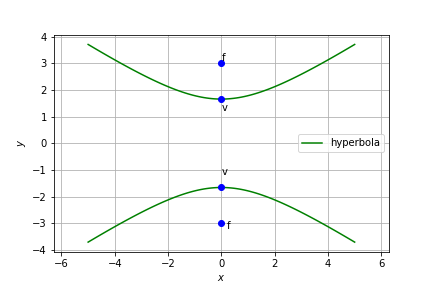
\includegraphics[width= \columnwidth]{assignment7.png}
    \caption{Hyperbola} \label{fig:1}
\end{figure}
\end{document}
